\documentclass{beamer}
\usepackage[utf8]{inputenc}
\usepackage{graphics}
\mode<presentation> {
\usetheme{unc}}
\setbeamertemplate{navigation symbols}{} % To remove the navigation symbols from the bottom of all slides uncomment this line

\usepackage{graphicx} % Allows including images
\usepackage{booktabs} % Allows the use of \toprule, \midrule and \bottomrule in tables


\usepackage{hyperref}
\hypersetup{linkcolor=blue,colorlinks=true}


% Remove symbols
\beamertemplatenavigationsymbolsempty


%\usetheme{default}

\usefonttheme{serif}

%----------------------------------------------------------------------------------------
%	TITLE PAGE
%----------------------------------------------------------------------------------------


\title[Monetary Policy]{\LARGE{Monetary Policy, Exchange Rates, and Currency Crises}}
\author[POLI 150]{Steven Saroka}
\institute{POLI 150}
\date{4 - 9 April 2024}


\begin{document}

\begin{frame}
\titlepage % Print the title page as the first slide
\end{frame}


%----------------------------------------------------------------------------------------
%	PRESENTATION SLIDES
%----------------------------------------------------------------------------------------

\begin{frame} 
	\frametitle{\LARGE{Announcements}}
	\begin{itemize}
		\Large{
			\item Exam 2 on April 18. Exact same format as Exam 1. Non-cumulative.
			\item PSSP module 2 open until April 10. See \href{https://tarheels.live/psspparticipants/}{PSSP site} for details, questions, and contact info.
			\item Prompt 10 due today (April 4).
			\item Prompt 11 due April 9.
		}
	\end{itemize}
\end{frame}

\begin{frame} 
	\frametitle{\LARGE{This Week's Class}}
	\begin{itemize}

			\item Domestic and international exchange rate impacts 
			\\~\\ 
			\item Bretton-Woods Monetary System
			\\~\\
			\item Monetary policy and currency devaluation
			\\~\\
			\item Balance of payments
			\\~\\
			\item Anatomy of a currency crisis
			\\~\\
			\item Application: Russia
			\\~\\ 		
			\item Application: Global Financial Crisis of 2008
		
	\end{itemize}
\end{frame}

\begin{frame} 
	\frametitle{\LARGE{Key Terms}}
	\begin{itemize}
		\item Exchange rate (fixed and floating)
		\item Appreciation/depreciation
		\item Inflation
		\item Monetary policy
		\item Mundell-Fleming Trilemma
		\item Current account
		\item Financial account
		\item Balance of payments
		\item Currency crisis
		\item Eurozone debt crisis
		\item Austerity
	\end{itemize}
\end{frame}


\begin{frame} 
\frametitle{\LARGE{Central Questions}}
\centering
\Large{How do currency relationships influence governments' decisions and their international relations? What are the causes and consequences of a currency crisis? What were the causes and consequences of the global financial crisis of 2008?}
\end{frame}

%% Currency map
\begin{frame}{\LARGE Currency Map}
    \centering
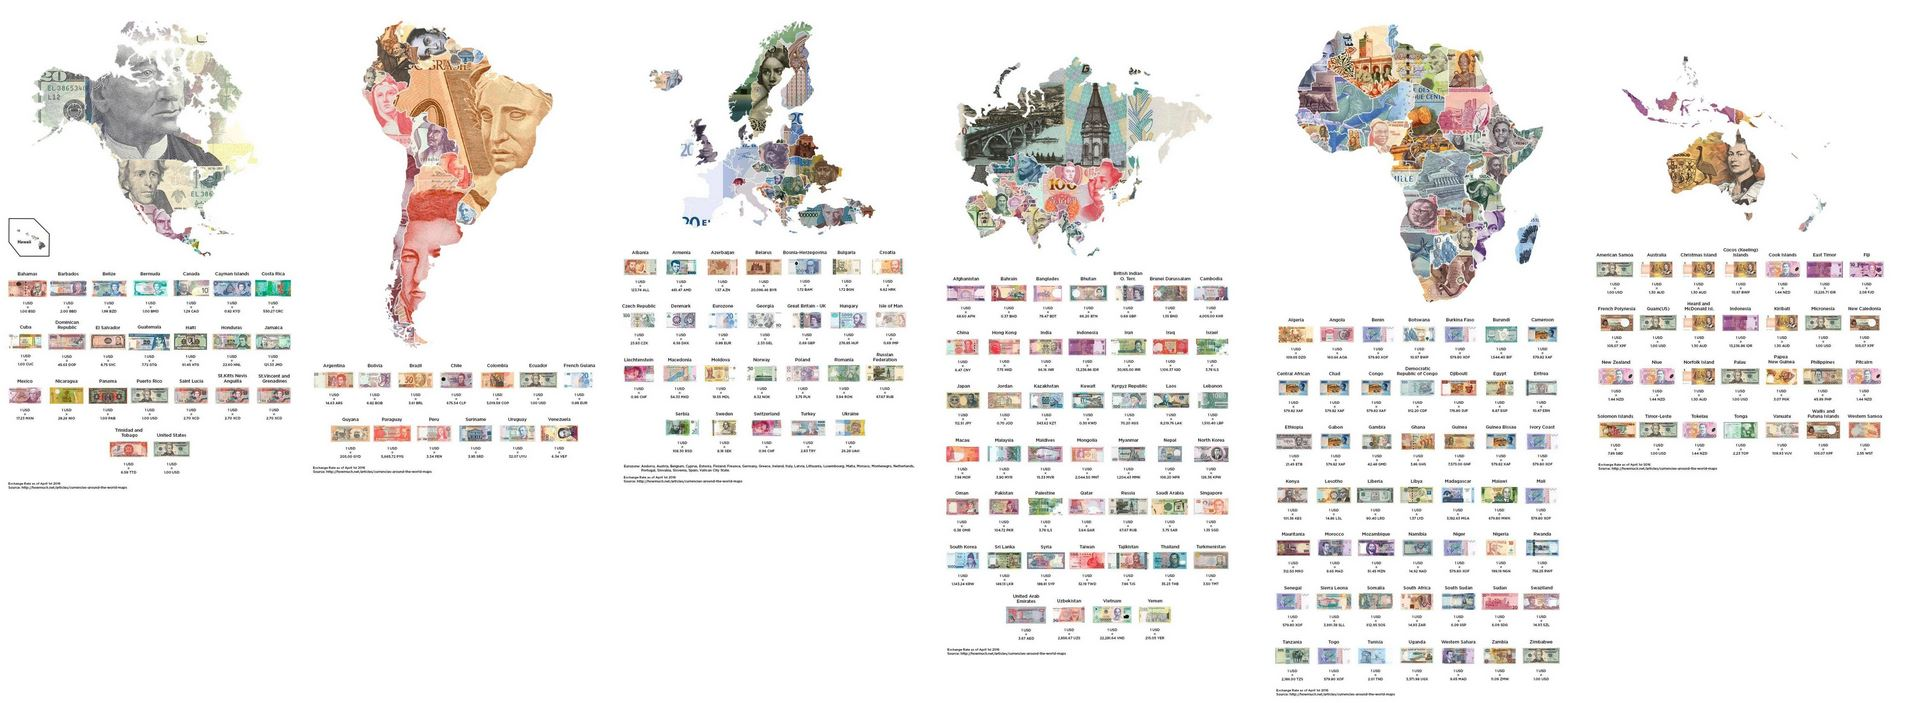
\includegraphics[width=\textwidth,height=0.8\textheight,keepaspectratio]{currency map.JPG}
\end{frame}

\begin{frame} 
	\frametitle{\LARGE{Introduction}}
	\begin{itemize}
			\item Thus far, we have discussed international financial relations without paying much attention to differences in currency across states. \pause
			\item However, state governments both issue their own currencies and affect the value of those currencies through their use of \textbf{monetary policy}:  supplying, controlling, and maintaining trust in a currency. \pause
			\item How is this possible? \textbf{Not all currencies are equally valued}.				
	\end{itemize}
\end{frame}

\begin{frame} 
	\frametitle{\LARGE{Introduction}}
	\begin{itemize}
		\item Most governments have their own currency (e.g. USD, Chinese yuan, British pound, etc.). \pause
		\item Some countries use another state's currency. \pause
		\begin{itemize}
			\item \href{https://www.investopedia.com/articles/forex/040915/countries-use-us-dollar.asp}{11 countries} use the USD. \pause 
		\end{itemize}
		\item Some common also currency arrangements exist (Euro, CFA Franc).  \pause
		\begin{itemize}
			\item Makes trading, investing across borders significantly easier. \pause 
		\end{itemize}	
		\item Why would a state choose one of these options over another? The choices made here are influenced by many considerations, but the most obvious is...
	\end{itemize}
\end{frame}


\begin{frame} 
	\frametitle{\LARGE{The Value of Money}}
	\begin{itemize}
		\item What is \$1 really worth, and why is it worth that? \pause
		\item One answer to this question is to compare the values of currencies to each other. \pause
		\item If I have \$1, how many British Pounds or Euros or Chinese Renmimbi/yuan can I get for that dollar? \pause
		\item This is formalized in the concept of the \textbf{exchange rate:} The price at which one currency is exchanged for another. 	
	\end{itemize}
\end{frame}

%values from google 
\begin{frame} 
	\frametitle{\LARGE{Exchange Rate Examples}}
\$1 is currently worth (at time of writing on 11/2):
	\begin{itemize}
		\item .94 Euros \pause
		\item 94.02 Russian rubles \pause
		\item 7.32 Chinese yuan \pause
		\item 1.37 Canadian dollars \pause
		\item 786.09 Nigeria naira \pause
	\end{itemize}
These values also change over time...
\end{frame}

\begin{frame}{\LARGE US Dollar Exchange Rate Over Time}
	\centering
	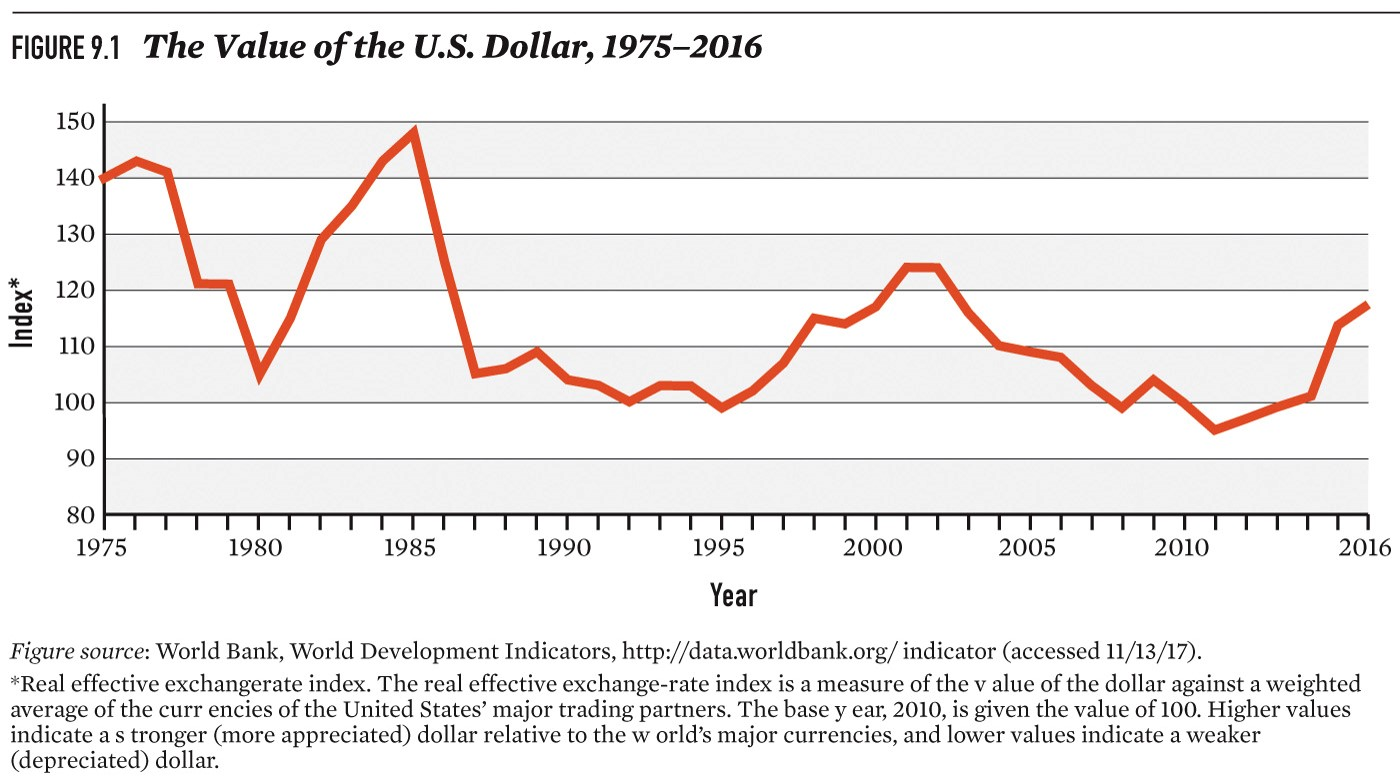
\includegraphics[width=\textwidth,height=0.8\textheight,keepaspectratio]{USXR.jpg}
\end{frame}

\begin{frame} 
	\frametitle{\LARGE{Exchange Rate Types}}
	The government chooses an \textbf{exchange rate regime} as part of its monetary policy:  \pause
	\begin{itemize}
		\item \textbf{Fixed:} the state commits to keeping its currency value tied to some other currency or commodity at a fixed rate. This means \textbf{the exchange rate never changes.} \pause 
		\item \textbf{Floating:} the state allows the currency to be traded on the open market without much control. This enables the exchange rate to fluctuate over time and with market conditions. \pause
	\end{itemize}
	\textbf{Most currencies today, and all major currencies like the USD, are floating.} The following examples implicitly assume a floating currency, as these are both more common and the most important currencies in the international system float.
\end{frame}

%% Exchange rate regimes 
\begin{frame}{\LARGE Exchange Rate Regimes}
	\centering
	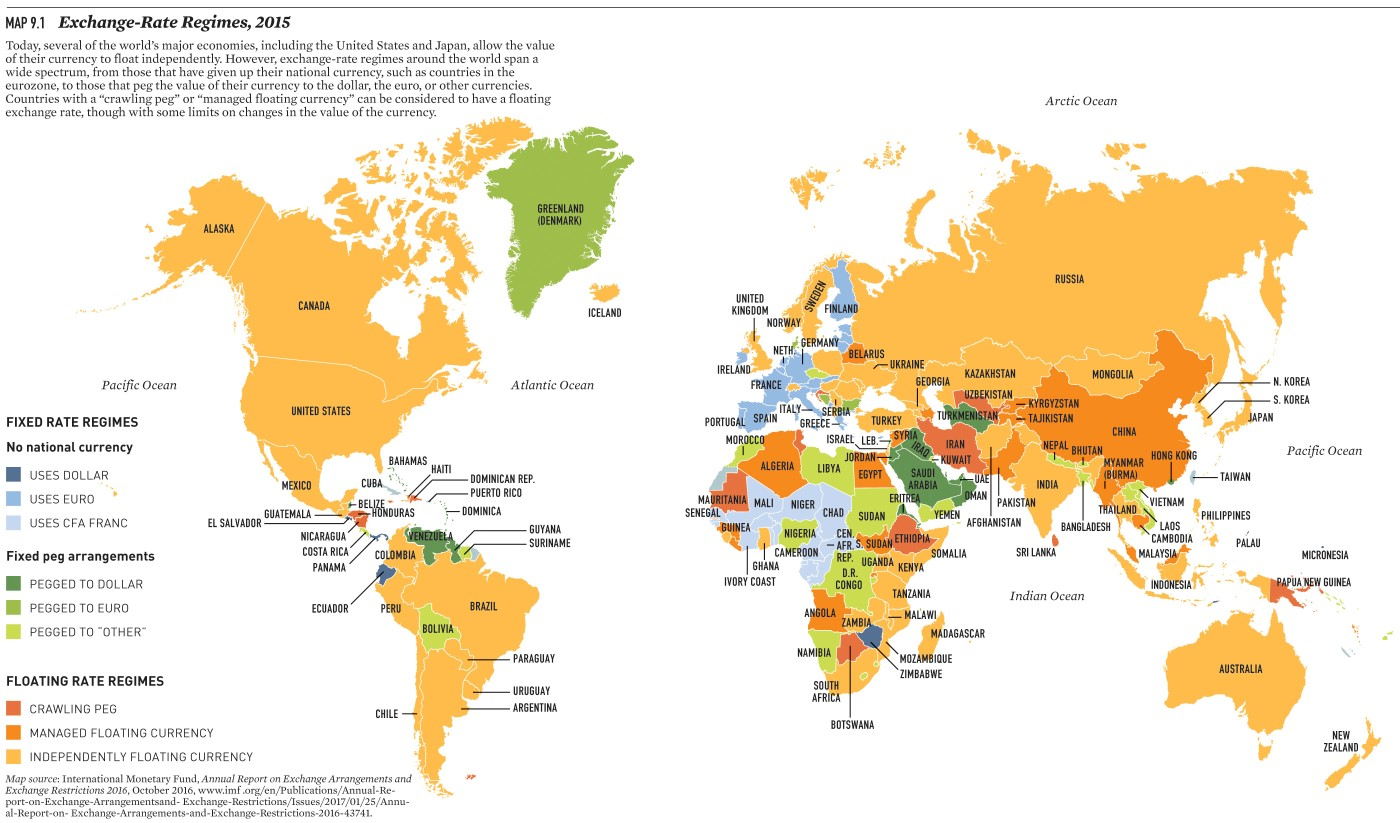
\includegraphics[width=\textwidth,height=0.8\textheight,keepaspectratio]{exchange rate regimes.jpg}
\end{frame}

\begin{frame} 
	\frametitle{\LARGE{Exchange Rates and Trade}}
	\begin{itemize}
		\item Why does this rate matter? Because international trade and investment very frequently involves the exchange rate. \pause
		\item To engage in economic activity in a given state, you need currency that state's businesses will accept. \pause
		\item In most cases, especially in developed rich states, this means converting your currency into their currency. \pause
		\item \textbf{Thus, changes in exchange rates have substantial implications for the profitability of international financial interactions.}
		\item Exchange rates are influenced by a variety of domestic and international factors.
	\end{itemize}
\end{frame}

\begin{frame} 
	\frametitle{\LARGE{Exchange Rates and Domestic Factors}}
	\begin{itemize}
		\item \textbf{Domestically, the value of money is itself subject to the laws of supply and demand.}
		\item As a running example, consider the US dollar (USD), which has a floating exchange rate.
		\item Consider \textbf{demand} for USD: what may make international investors want more USD? \pause
		\item Investment opportunities in the US (loans to US businesses), desire to buy export goods from the US, etc. -- any economic activity that involves the USD increases demand for it.
	\end{itemize}
\end{frame}

\begin{frame} 
	\frametitle{\LARGE{Exchange Rates and Domestic Factors}}
	\begin{itemize}
		\item These investment opportunities in America increase demand for dollars, especially if the interest rates for loans are profitable. \pause
		\item So, investors need to trade some of their currency for some USD to invest. \pause
		\item However, the supply of dollars is finite. \pause
		\item \textbf{As more investors want to invest in an economy, they will drive up demand for that country’s currency, giving it a higher value in comparison to their own.}
		\item This increase is \textbf{appreciation}. Currencies \textbf{appreciate/strengthen} when they increase in value relative to other currencies. 
	\end{itemize}
\end{frame}

\begin{frame} 
	\frametitle{\LARGE{Exchange Rates and Domestic Factors}}
	\begin{itemize}
		\item Consider the \textbf{supply} of money. Where does the USD, or any other currency, come from? \pause \textbf{Governments create and maintain it.} \pause
		\item \textbf{Monetary policy} refers to actions governments take to affect the amount of their currency circulating in the economy. \pause
		\item This is primarily done via raising and lowering interest rates set by that state's central bank (in the US, the Federal Reserve). \pause
		\item Central bank interest rate changes are mirrored by the biggest banks, and then eventually filtered down to individual consumers. 
	\end{itemize}
\end{frame}

\begin{frame} 
	\frametitle{\LARGE{Exchange Rates and Domestic Factors}}
	\textbf{Lower} interest rates \textbf{increase} the money supply.
		\begin{itemize}
			\item Lower interest rates mean cheaper borrowing. \pause
			\item Cheaper borrowing means fewer incentives to keep money sitting in savings accounts. \pause
			\item This means a net increase in the amount of money in the economy.
			\item \textbf{Holding other factors constant (no concurrent increase in demand), this increase in supply decreases the value of money.}
			\item This decrease is \textbf{depreciation}. Currencies \textbf{depreciate/weaken/devalue} when they decrease in value relative to other currencies. 
		\end{itemize}
\end{frame}

\begin{frame} 
	\frametitle{\LARGE{Exchange Rates and Domestic Factors}}
	\textbf{Higher} interest rates \textbf{decrease} the money supply.
	\begin{itemize}
		\item Higher interest rates mean borrowing is now more expensive. \pause
		\item More expensive borrowing means more incentives to save money. \pause
		\item This means a net decrease in the amount of money in the economy.
		\item \textbf{Holding other factors constant (no concurrent increase in demand), this decrease in supply increases the value of money.} This is \textbf{appreciation}.
	\end{itemize}
\end{frame}

\begin{frame} 
	\frametitle{\LARGE{Why Engage in Monetary Policy?}}
	\begin{itemize}
		\item Why may states want to change the interest rate? \pause
		\item Suppose that the economy is starting to slow. Politicians are worried that this could lead to unemployment or recession. \pause
		\item Lower interest rates mean more money in circulation, which means more demand by consumers and investment by businesses, ultimately stimulating growth and preventing a recession. \pause
	\end{itemize}
\end{frame}


\begin{frame} 
	\frametitle{\LARGE{Why Engage in Monetary Policy?}}
	\begin{itemize}
		\item Obvious question: economic growth is great, so why not always keep interest rates low? 
		\item If there is too much money in circulation, but not enough production of goods and services to match this increased demand, what happens? \pause Prices rise.
		\item This causes \textbf{inflation}: the ability of currency to convert itself to real goods and services decreases as prices rise. \pause
		\item Thus, for governments worried about inflation, they may choose to raise interest rates.	
		\item The correct interest rate is a balancing act for the government.
	\end{itemize}
\end{frame}

\begin{frame}{\LARGE Inflation Example}
	\centering
	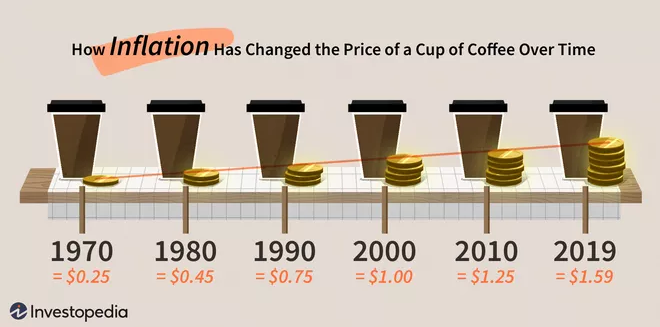
\includegraphics[width=\textwidth,height=0.8\textheight,keepaspectratio]{coffeeinflation.png}
\end{frame}

\begin{frame} 
	\frametitle{\LARGE{Fixed Exchange Rates}}
	\begin{itemize}
		\item Prior examples assumed a floating rate. What about fixed rates? \pause
		\item Fixed rates generate stable expectations about trade and international investment, and political scientists have found that they encourage international investment and trade. \pause 
		\item However, governments on fixed rates have committed to a specific value, \textbf{even if changing it would improve the domestic economy}. \pause
		\begin{itemize}
			\item Recall previous example about a potential recession. A fixed rate means the state \textbf{cannot} try to influence the exchange rate. \pause
		\end{itemize}
		\item Fixed rates reduce policy options in response to financial turbulence, but provide extra stability when markets are calm.
	\end{itemize}
\end{frame}

\begin{frame} 
	\frametitle{\LARGE{Currency and International Investment}}
	\begin{itemize}
		\item Governments also must consider international investments when deciding on their monetary policy. \pause
		\item Changing the supply of money not only impacts domestic actors, but also international investors, via the exchange rate. \pause
		\item Currencies \textbf{appreciate/strengthen} when they increase in value relative to other currencies. \pause
		\item Currencies \textbf{depreciate/weaken/devalue} when they decrease in value relative to other currencies. \pause
		\item \textbf{Changes to the interest rate are the primary way state governments can impact the exchange rate.}		
	\end{itemize}
\end{frame}

\begin{frame} 
	\frametitle{\LARGE{Currency and International Investment}}
	\begin{itemize}
		\item Why does an increase in the interest rate lead to appreciation? \pause
		\item There is less money in the economy, as domestic actors tend to save money, shrinking the amount of money circulating. Supply decreases. \pause
		\item At the same time, more international investors want to invest due to those higher interest rates, increasing demand for the currency. \pause
		\item This makes the currency more valuable, and so it strengthens in comparison to other currencies being traded for it. \pause
		\item Depreciation is this story in reverse.
	\end{itemize}
\end{frame}

\begin{frame} 
	\frametitle{\LARGE{Strong Currency Trade Example}}
	Say you want to buy Italian leather shoes, currently retailing for 100 Euros, with a USD:Euro exchange rate of 1:1.
	\begin{itemize}
		\item With that exchange rate, those shoes will cost you \$100. \pause 
		\item Say the dollar now appreciates, such that the exchange rate is 1:2 (\$1 now gets you 2 euros). \pause
		\item Now, that shoe only costs you \$50.
		\item If you are a shoe shop in the US, you can now import more of those shoes for the same amount than before. \pause
		\item By the same logic, US exports are now more expensive for Italian consumers who must convert their Euros into USD to buy them. \pause
	\end{itemize}
	A weakened dollar would lead to the reverse of this situation.
\end{frame}

\begin{frame} 
	\frametitle{\LARGE{Exchange Rate and Intl Trade}}
The relationships between currencies inform the costs of trade. \pause
	\begin{itemize}
		\item When a state's currency is strong, it can import more but export less. \pause
%		\begin{itemize}
%			\item 1981-1985: USD appreciated by more than 50\% $\rightarrow$ greater prosperity for consumers $\rightarrow$ 1.5 million manufacturing jobs lost \pause
%		\end{itemize} 
		\item When a state's currency is weak, it can import less but export more easily.
		\item Stronger currency is good for consumers of imported goods, but import-competing industries and exporting industries in that state find it decreases their competitiveness. \pause
		\item Weaker currency is good for import-competing industries and exporting industries, but tends to be worse for the buying power of consumers. 
	\end{itemize}

\end{frame}

\begin{frame} 
	\frametitle{\LARGE{Exchange Rate and Intl Trade}}
	The relationships between currencies inform the costs of trade. \pause
	\begin{itemize}
		\item Example: USD appreciated by more than 50\% from 1981-1985.
		\item This led to greater prosperity (purchasing power) for American consumers. 
		\item At the same time, 1.5 million American manufacturing jobs were lost as American goods became more expensive to global consumers. \pause 
	\end{itemize}
	\textbf{Monetary policy is driven as much by which groups can effectively lobby the government for changes in monetary policy as by purely economic concerns.}	
\end{frame}

\begin{frame} 
	\frametitle{\LARGE{Domestic Politics and Exchange Rates}}
	\begin{itemize}
		\item Like all other economic policies, exchange rates produce winners and losers domestically. \pause 
		\item Thus, if the economy relies on exports, there will be pressure to fix or manage the exchange rate so that the currency stays weak. \pause 
		\item Whereas if the economy relies on imports, there may be more pressure for looser capital and interest rate controls so that the currency can appreciate. \pause
		\item Collective action problems are present here, meaning that relative group size matters, with industries usually having an organizational edge over consumers. 
	\end{itemize}
\end{frame}

\begin{frame}{\LARGE Bretton Woods Monetary System}
	\centering
	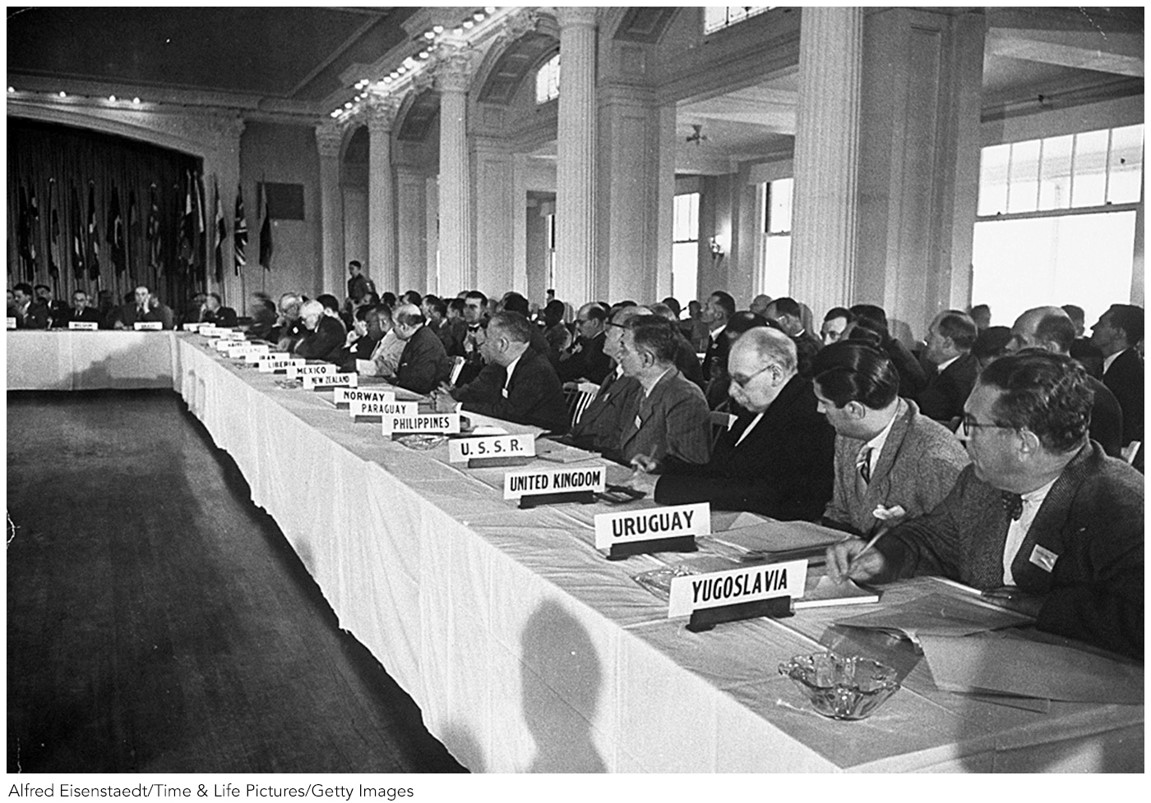
\includegraphics[width=\textwidth,height=0.8\textheight,keepaspectratio]{Brettonwoods.jpg}
\end{frame}

\begin{frame} 
	\frametitle{\LARGE{Bretton Woods Monetary System}}
	\begin{itemize}
		\item Following WWII, there was a general consensus that encouraging international trade and investment would both help general economic recovery and make interstate war less likely. \pause
		\item Fixed exchange rates were known to encourage international trade and investment, but states also remembered the political problems created by fixed exchange rates during the British gold standard era.	\pause
		\item The solution was a combination of fixed and floating rates.
	\end{itemize}
\end{frame}

\begin{frame} 
	\frametitle{\LARGE{Bretton Woods Monetary System}}
	\begin{itemize}
		\item The USD would be fixed to gold at a rate of \$35/ounce, with other states' currencies fixed to the US dollar but allowed to occasionally adjust that fixed rate if economic conditions called for it. \pause
		\item The IMF originally served as the arbiter of whether a state could adjust its rate in this system. The GATT served to lower protectionist trade barriers, while the World Bank provided reconstruction loans. \pause
		\item \textbf{This system was stable so long as the dollar's value stayed fixed.}
	\end{itemize}
\end{frame}

\begin{frame} 
	\frametitle{\LARGE{Bretton Woods Monetary System}}
	\begin{itemize}
		\item By the early 1970s, US government borrowing to fund the Vietnam war and assorted Great Society social programs meant there were very clearly more dollars in circulation than the US had gold to exchange them for. \pause
		\item Many investors (and states) began asking the US government to exchange their dollars for gold. \textbf{Remember, this is the fundamental underlying promise of the whole Bretton-Woods arrangement.} \pause
		\item By 1971, President Nixon has a choice:
		\begin{itemize}
			\item Stop spending money/raise taxes (austerity) to reduce supply of dollars to maintain the fixed rate.
			\item Break promise to convert dollars to gold.
		\end{itemize}		
	\end{itemize}
\end{frame}

\begin{frame} 
	\frametitle{\LARGE{The Fall of Bretton Woods}}
	\begin{itemize}
		\item Nixon does the latter, unilaterally taking the US off the gold standard. \pause
		\item US economy weakens in the following years, interest rates begin to rise, and the purchasing power of the dollar is threatened. Foreign crises and an OPEC oil embargo do not help. \pause
		\item To prop up the dollar, US foreign policy shifts towards convincing OPEC states, in particular Saudi Arabia, to sell oil in dollars.	\pause
		\item This both creates the petrodollar system and ensures the primacy of the dollar in the international economy even after Bretton-Woods (see next week's Bapat (2019) reading for details). 
	\end{itemize}
\end{frame}

\begin{frame} 
	\frametitle{\LARGE{Intl Governance of Exchange Rates}}
	\begin{itemize}
			\item The post-BW world is mostly a floating rate world.
			\item In this post-BW world, governments have incentives to cooperate... \pause
			\begin{itemize}
				\item Want to prevent excessive swings in currency value \pause 
				\item Stop contagion of crises \pause 
				\item Avoid competitive devaluations  \pause
			\end{itemize}
			\item ... but may struggle to work together \pause
			\begin{itemize}
				\item They'd prefer other countries to commit to fixed rates which favor their own trade \pause 
				\item Might engage in competitive devaluations  
			\end{itemize}
		
	\end{itemize}
\end{frame}

\begin{frame} 
	\frametitle{\LARGE{Intl Governance of Exchange Rates}}
	\begin{itemize}
		\item During the Bretton-Woods era, the IMF was in charge of managing currency relationships. \pause
		\item Today, the IMF coordinates some responses, but there is largely little formal cooperation on international exchange rates, as  major currencies float. \pause 
		\item Many countries influence their currencies indirectly through interest rates. \pause 
		\item Other countries may more explicitly interfere with their rates via devaluation or currency manipulation.		
	\end{itemize}
\end{frame}


\begin{frame} 
	\frametitle{\LARGE{Monetary Policy Choices}}
	This discussion shows that states can directly control monetary policy in three possible ways:
	\begin{itemize}
		\item \textbf{Interest rates:} creating a central bank to control the domestic supply of currency by setting interest rates. \pause 
		\item \textbf{Capital controls:} allowing money to flow freely across its borders (or preventing it from doing so). \pause 
		\item \textbf{Exchange rates:} choosing to fix its currency to something (e.g. gold standard), or to let it float. \pause 
		\item However, states can only choose two of these three policy options. \pause 
		\begin{itemize}
			\item Thus, this is known as the \textit{Mundell-Fleming Trilemma} \pause
			\item \href{https://www.youtube.com/watch?v=yt0m7N3bqXM}{A quick overview of the logic behind this} 
		\end{itemize}
	\end{itemize}
\end{frame}

% Trilemma slide 
\begin{frame}{\LARGE Trilemma}
	\centering
	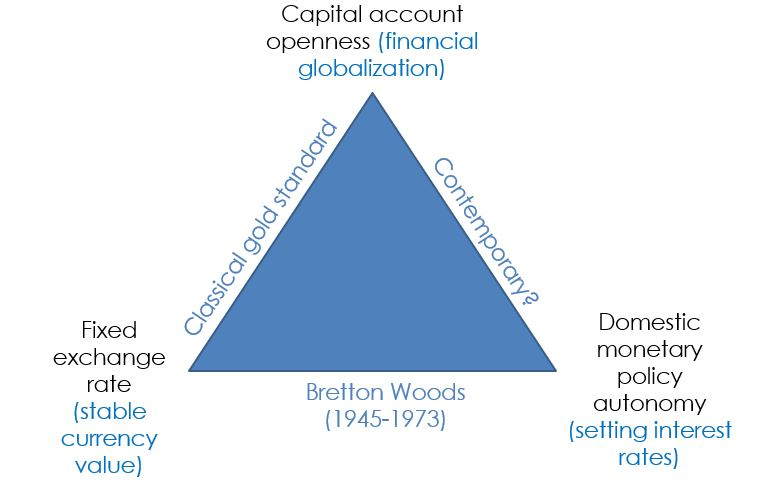
\includegraphics[width=\textwidth,height=0.8\textheight,keepaspectratio]{trilemma.JPG}
\end{frame}



\begin{frame} 
	\frametitle{\LARGE{Currency Manipulation}}
	\begin{itemize}
			\item Some states purposely keep their currencies weak to stimulate exports. \pause
			\item When countries intentionally depreciate their currency, this is known as \textbf{devaluation} or \textbf{currency manipulation}. \pause 
			\item China post-1979 weakened the renminbi/yuan to benefit its exporters and international consumers to great financial success, despite effectively taxing its own domestic consumers.  \pause
			\item This practice causes friction with international trading partners who face backlash from their own domestic producers, who argue their international competitors are essentially getting government help. 
	\end{itemize}
\end{frame}

% USD-CNY conversion
\begin{frame}{\LARGE CNY-USD Conversion}
	\centering
	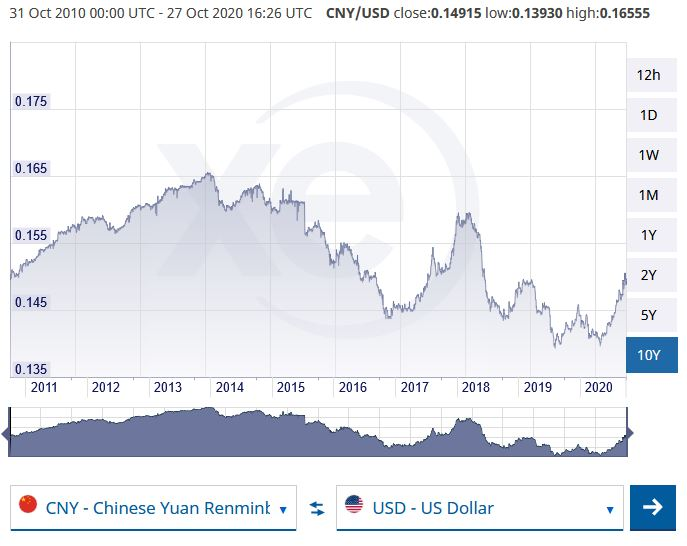
\includegraphics[width=\textwidth,height=0.8\textheight,keepaspectratio]{USD to CNY conversion.JPG}
\end{frame}

\begin{frame} 
	\frametitle{\LARGE{Currency Manipulation}}
		\begin{itemize}
			\item Currency manipulation has been particularly problematic for US-China trade relationship, given the dependence of these two economies on each other. \pause 
			\item China is widely acknowledged to have manipulated currencies from 2003-2013. \pause 
			\item President Trump named China a currency manipulator in August 2019, then revoked this in January 2020; this appeared to be a tactic in the then-ongoing US-China trade war rather than an independently verified fact. \pause
			\item Unclear economic benefits from these accusations, which may explain why the US did not formally label China a currency manipulator from 2003-2013.
		\end{itemize}	
\end{frame}



\begin{frame} 
	\frametitle{\LARGE{Balance of Payments}}
	Monetary policy also impacts a state's Balance of Payments.
	\begin{itemize}
		\item A state's net trade (imports minus exports) is known as the \textbf{current account}. \pause
		\item A state's net investments (inflows minus outflows) are known as the \textbf{financial account}. \pause
		\item When a state imports more than it exports, it must bring in new foreign investments to pay for the imports. \pause 
		\item The financial and current accounts should balance out to 0 (thus, known as the \textbf{balance of payments}). 
	\end{itemize}
\end{frame}

%% US China Current account
\begin{frame}{\LARGE US-China Current Accounts}
	\centering
	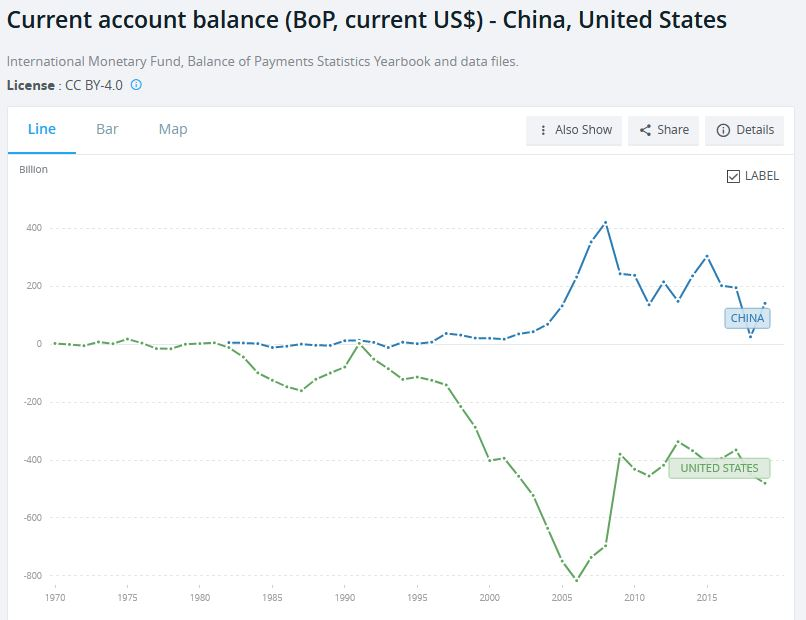
\includegraphics[width=\textwidth,height=0.8\textheight,keepaspectratio]{US-China current account.JPG}
\end{frame}

%% US China financial account 
\begin{frame}{\LARGE US-China Financial Accounts}
	\centering
	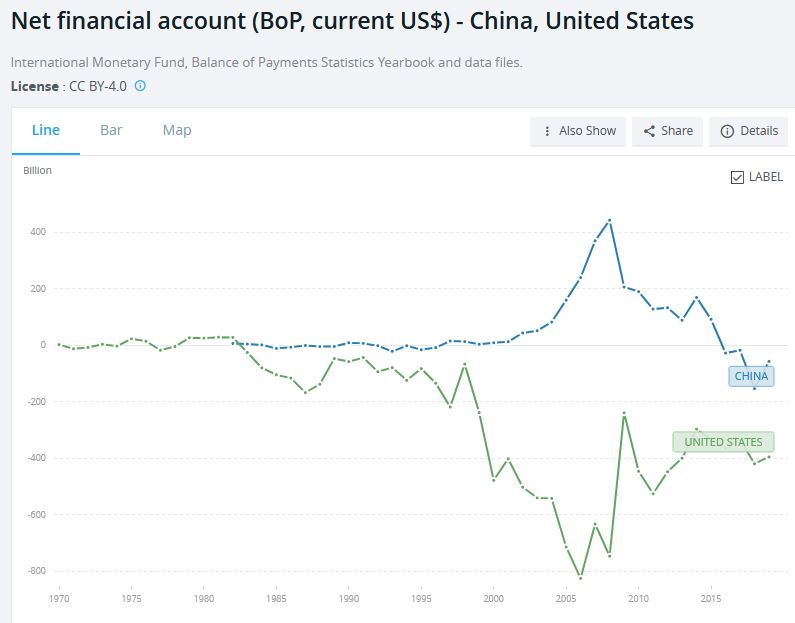
\includegraphics[width=\textwidth,height=0.8\textheight,keepaspectratio]{US-China financial account.JPG}
\end{frame}

\begin{frame} 
	\frametitle{\LARGE{Balance of Payments}}
	\begin{itemize}
		\item \textbf{By definition, current accounts and financial accounts should balance each other (sum to 0).} \pause
		\item Why? For every trade import coming into the state, there must be an outflow of capital to pay for it. \pause
		\item Example: if I import \$100 of goods from a foreign producer, then I am sending \$100 of my currency (filtered through the exchange rate) abroad to that foreign producer. \pause
		\item During normal economic activity, this balance holds, and international trade and investment continues as normal. 
	\end{itemize}
\end{frame}

\begin{frame} 
	\frametitle{\LARGE{Currency Crisis}}
	\begin{itemize}
		\item A \textbf{balance of payments crisis/currency crisis} occurs when this balance is disrupted. \pause
		\item In a currency crisis, the current account and financial account no longer sum to 0. \pause
		\item Substantively, this means that the state's economy is unable to continue to pay for imports and/or make timely repayments on its foreign debt. 
	\end{itemize}
\end{frame}

\begin{frame} 
	\frametitle{\LARGE{Anatomy of a Currency Crisis}}
	\begin{itemize}
		\item Step 1: develop a \textbf{current account deficit}: the total value of the goods and services that are entering the economy exceeds the value that the state's economy is exporting. \pause
		\item A current account deficit is not intrinsically bad, so long as the state's economy is able to pay for these incoming goods/services by attracting some inward flow of foreign capital.
	\end{itemize}
\end{frame}

\begin{frame} 
	\frametitle{\LARGE{Anatomy of a Currency Crisis}}
	\begin{itemize}
		\item Step 2: lose the ability to pay off that current account deficit. How? \pause
		\item Foreign creditors become concerned about debt repayment, setting off a financial crisis. Financial and currency crises are often linked. \pause
		\item As a part of this, these creditors try to remove their money from the economy to avoid losing their investments. This is a sudden increase in \textbf{outbound capital flows}. \pause
		\item A financial crisis is now also occurring concurrently with everything else described here.	
	\end{itemize}
\end{frame}

\begin{frame} 
	\frametitle{\LARGE{Anatomy of a Currency Crisis}}
	\begin{itemize}
		\item Step 3: the state's currency begins to devalue. Why?
		\item Those outbound capital flows mean that investors are now converting their previous holdings from the state's economy (which were in the state's currency) back into the currency of their home state.
		\begin{itemize}
			\item Note this assumes a floating exchange rate.
			\item The same thing can happen with a fixed rate, if international investors believe the fixed rate is no longer credible. \pause
		\end{itemize}
		\item \textbf{This means a massive devaluation of the currency as the currency supply suddenly drastically increases.}
	\end{itemize}
\end{frame}

\begin{frame} 
	\frametitle{\LARGE{Anatomy of a Currency Crisis}}
	Step 3 continued:
	\begin{itemize}
		\item Feedback loops and contagion effects begin to take hold.
		\item Other international investors observe this initial capital outflow, get scared about their investments, and move to pull their funds out too. \pause
		\item Domestic consumers may also panic and try to remove their money for savings or convert it into foreign currency that is perceived as safer, exacerbating this.
		\item \textbf{This devaluation is especially bad for domestic groups that have borrowed money in foreign currency, as it is now more expensive to repay those loans.}
	\end{itemize}
\end{frame}

\begin{frame} 
	\frametitle{\LARGE{Anatomy of a Currency Crisis}}
	\begin{itemize}
		\item Step 4: the state's central bank fights back by utilizing its \textbf{foreign reserves}, which are its holdings of foreign currency. \pause
		\item The central bank attempts to use that foreign currency to buy back its own currency, in an attempt to decrease the supply and thereby prop up the value of its currency. \pause
		\item At this point, the central bank is essentially fighting market forces over the value of the state's currency. \pause
		\item Step 4a: if the central bank is successful and stabilizes the currency, then the crisis is over. If it fails to do so...
	\end{itemize}
\end{frame}

\begin{frame} 
	\frametitle{\LARGE{Anatomy of a Currency Crisis}}
	\begin{itemize}
		\item Step 5: the state's currency is in free-fall as investors dump their holdings.
		\item Remember that a financial crisis is now also occurring as domestic borrowers (possibly including the government) are now struggling to repay loans denominated in foreign currency. Domestic firms may start to go bankrupt, creating further economic turmoil.  \pause
		\item The state's central bank can try to raise interest rates, while the government can implement austerity measures, but both of these steps will have negative domestic economic impacts.
		\item These crises are usually resolved with some kind of bailout and/or structural adjustment program.
	\end{itemize}
\end{frame}

\begin{frame} 
	\frametitle{\LARGE{Application: Russia}}
	\begin{itemize}
		\item Since the Russian invasion of Ukraine, the US and various Western allies have imposed a range of sanctions on Russia. \pause
		\item They have been joined by private corporations voluntarily withdrawing from Russian markets. \pause
		\item This is a general understanding, but what specifically is going on, and why are these sanctions so damaging?
	\end{itemize}
\end{frame}

\begin{frame} 
	\frametitle{\LARGE{Targeted Sanctions}}
	America's sanctions have taken a multi-pronged approach (some details from \href{https://www.vox.com/22968949/russia-sanctions-swift-economy-mcdonalds}{here}):
	\begin{itemize}
		\item Personal targeted sanctions against Putin and assorted Russian government officials and oligarchs. \pause
		\item These mean that any of their assets in the international banking system are now frozen, while it is illegal for Americans to do any form of business with them.
		\item These may hurt these oligarchs to some degree, but these are not the primary source of Russia's financial pain.
	\end{itemize}
\end{frame}

\begin{frame} 
	\frametitle{\LARGE{General Sanctions}}
	Of more importance are the sanctions targeted against the Russian economy:
	\begin{itemize}
		\item The primary means here has been US sanctions against the Russian central bank, which include freezing any foreign reserves held in the US financial system.
		\begin{itemize}
			\item The EU implemented a similar plan. \pause
		\end{itemize}
		\item The US has also frozen the assets of other Russian banks in the US banking system, while blocking Russian corporations from accessing US markets for stocks and bonds, and targeting Russian defense firms that would import goods necessary for a sustained war effort. \pause
		\item The Biden administration also banned imported Russian oil, natural gas, and coal from US markets. \pause
		\item EU implemented similar import bans, with some exceptions for states dependent on these imports.
	\end{itemize}
\end{frame}

\begin{frame} 
	\frametitle{\LARGE{Removal from SWIFT}}
	\begin{itemize}
		\item The US and EU removed the most of the Russian banking sector from SWIFT, the messaging system that details cross-border payments between banks. \pause
		\item There is no short-term alternative to using SWIFT, making this tantamount to ripping the Russian banking sector out of the global economy.
		\item This means that Russian banks are effectively unable to transfer currency into or out of the country.
	\end{itemize}
\end{frame}

\begin{frame} 
	\frametitle{\LARGE{EU and Other Sanctions}}
	\begin{itemize}
		\item Meanwhile, the EU has coordinated its sanctions, implementing many similar ones to the US (with one exception being continued payments to Russia for natural gas required by European markets). \pause
		\item This means that there are very few loopholes for Russian firms to evade these sanctions. \pause
		\item Meanwhile, many MNCs have also suspended or ended operations in Russia of their own volition (likely influenced by the difficulty of actually getting profits out of Russia given these sanctions).
	\end{itemize}
\end{frame}

\begin{frame} 
	\frametitle{\LARGE{Cumulative Effects}}
	\begin{itemize}
		\item In the short-term, the most economically painful impact came from the sanctions targeted at Russia's central bank. \pause
		\item Without access to its foreign reserves, it could not fight the devaluation of the ruble as investors withdrew their investments in response to these sanctions, while ordinary Russians moved to convert their rubles to safer currencies (like the dollar). \pause
		\item This meant a massive, swift, and brutal currency crisis for Russia \textbf{with the central bank effectively powerless to fight it}. 
	\end{itemize}
\end{frame}

%https://www.xe.com/currencycharts/?from=USD&to=RUB&view=1Y
\begin{frame}{\LARGE USD:RUB Exchange Rate}
	\centering
	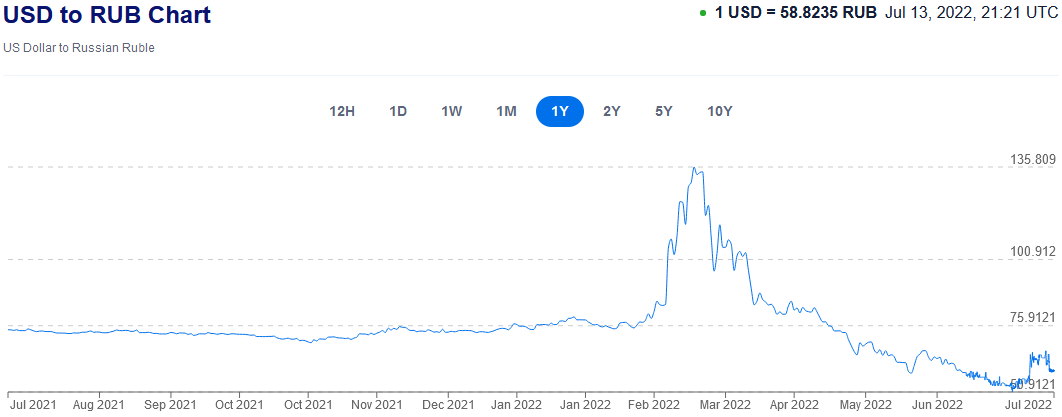
\includegraphics[width=\textwidth,height=0.9\textheight,keepaspectratio]{USDRUB.png}
\end{frame}

\begin{frame} 
	\frametitle{\LARGE{Cumulative Effects}}
	\begin{itemize}
		\item Meanwhile, a similarly swift financial crisis mounted as the isolation of the Russian financial sector devastated investor confidence in the Russian economy in general. \pause
		\item This exchange rate also means that Russian businesses holding foreign-denominated debt will find it virtually impossible to pay off. \pause
		\item Investors know that, and know that Russian firms may be unable to make their payments even if they want to, due to the isolation of Russia's financial system. \pause
		\item End result: a currency crisis leading to general financial crisis, but with several major actors in the global economy doing their best \textbf{to make the situation worse}.
	\end{itemize}
\end{frame}

\begin{frame} 
	\frametitle{\LARGE{Russian State Initial Responses}}
	\begin{itemize}
		\item Central bank has attempted to prop up the currency, while also briefly pushing interest rates to 20\% (\href{https://www.npr.org/2022/02/28/1083478065/russias-central-bank-doubles-a-key-interest-rate-as-sanctions-spark-economic-tur}{source}) before reverting to pre-war levels (\href{https://www.cnbc.com/2022/06/10/russia-cuts-key-interest-rate-back-to-pre-war-level.html}{source}). \pause
		\item Russian government forced corporations to exchange what foreign reserves they have for rubles, to get access to some foreign currency (\href{https://www.whitehouse.gov/briefing-room/statements-releases/2022/03/24/fact-sheet-united-states-and-allies-and-partners-impose-additional-costs-on-russia/}{White House press release}). \pause
		\item Moscow stock exchange closed from Feb. 26 - Mar. 24, 2022, reopening with heavy restrictions (details \href{https://fortune.com/2022/03/24/russia-stock-market-reopen-moex-month-offline/}{here}). \pause
	\end{itemize}
	\textbf{The takeaway: the Russian government's responses are simply insufficient to prevent severe economic damage, despite the \href{https://www.nytimes.com/2022/04/04/opinion/ruble-value.html}{ruble's rebound in April}.}
\end{frame}

\begin{frame} 
	\frametitle{\LARGE{Russian State Longterm Responses}}
	\begin{itemize}
		\item Ongoing and aggressive measures to prevent capital flight combined with high energy prices to paradoxically make the ruble, arguably, the world's strongest currency (\href{https://www.cbsnews.com/news/russia-ukraine-ruble-currency-russian-economy-sanctioms-2022/}{source}) in 2022. Technically. \pause
		\item Russian economy shrunk in 2022 and expected to continue, but has held up better than expected. \pause
		\item June 2022 Russian debt default due to sanctions preventing it from repayment (\href{https://www.cbsnews.com/news/russia-default-on-debt/}{source}). \pause
		\item Russian economy is hurting on all measures (\href{https://www.bbc.com/news/world-europe-60125659}{source}), but has been surprisingly resilient and has avoided the complete collapse predicted initially.
	\end{itemize}
	
\end{frame}

\begin{frame} 
	\frametitle{\LARGE{Notable Takeaways}}
	There are several remarkable aspects of this international response:
	\begin{itemize}
		\item Speed of sanction implementation. \pause
		\item Scale of sanctions and restrictions on the Russian economy. \pause
		\item Level of international cooperation on these sanctions. \pause
		\item Goal of these sanctions: a concerted effort to hurt the Russian economy, effectively cutting off a major market from the rest of the world.	
	\end{itemize}
\end{frame}

\begin{frame} 
	\frametitle{\LARGE{Introduction to the 2008 Financial Crisis}}
	\begin{itemize}
		\item The 2008 global financial crisis is one of, if not the, defining financial events of the post-Cold-War era. \pause
		\item It was also responsible for the Eurozone debt crisis, a similarly important financial event. \pause
		\item These crises and their consequences are important for understanding the global economic environment. 
	\end{itemize}
\end{frame}

\begin{frame} 
	\frametitle{\LARGE{2008 Financial Crisis}}
	\begin{itemize}
		\item The 2008 Financial Crisis has several names: 2007-2010 Financial Crisis, the Great Recession. \pause
		\item It involved a 2008 stock market collapse saw the loss of \$14 \textbf{trillion}, equal to America's entire GDP. \pause
		\item Global equity losses totaled \$35 trillion. That's equal to the combined GDPs of the U.S., EU, and Japan. \pause
		\item Alan Greenspan, former chair of the Federal Reserve, described it as “Likely to be judged as the most virulent global financial crisis ever.” \pause
		\item Was it worse than the Great Depression? Probably not, but still very bad...	
	\end{itemize}
\end{frame}


\begin{frame}{\LARGE Recession Job Losses}
	\centering
	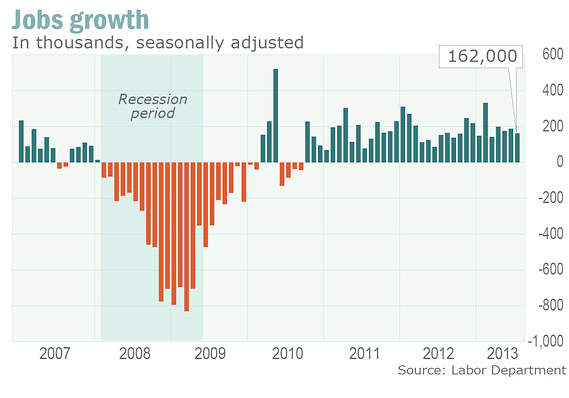
\includegraphics[width=\textwidth,height=.8\textheight,keepaspectratio]{jobgrowth.png}
\end{frame}

\begin{frame}{\LARGE Recession Equity Market Contract}
	\centering
	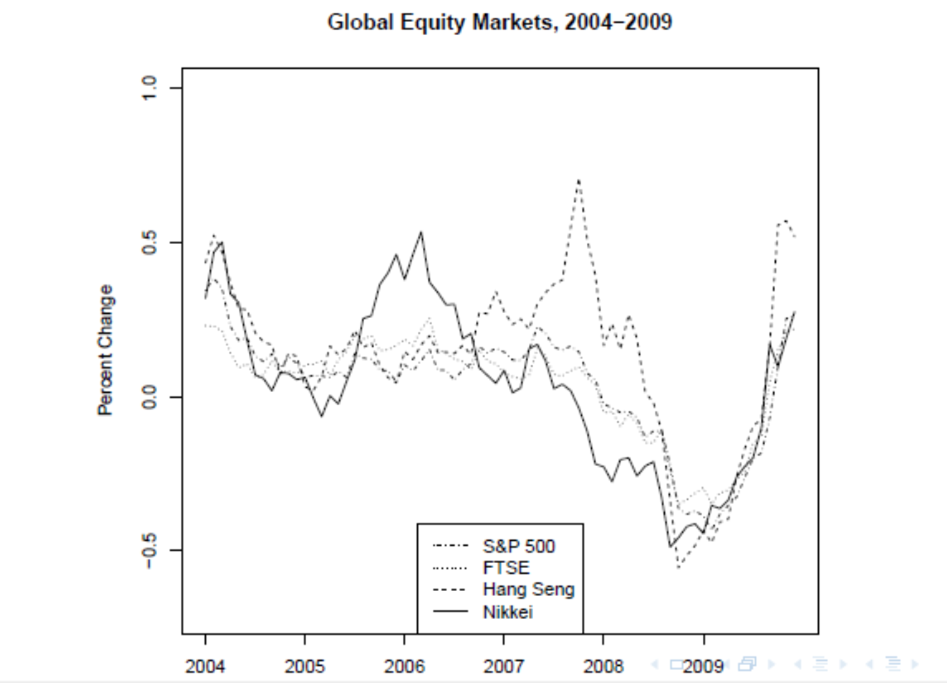
\includegraphics[width=\textwidth,height=.8\textheight,keepaspectratio]{globalequity.png}
\end{frame}

\begin{frame} 
	\frametitle{\LARGE{Background: US Economy}}
	Understanding this crisis requires a close look at the American economy in the years prior to 2008. \pause
	\begin{itemize}
		\item The Bush administration implements tax cuts, and encourages the Federal Reserve to reduce interest rates. \pause
		\item The US government is also borrowing more to finance the wars in Afghanistan and  Iraq. \pause	
		\item This means an increase in the US current account deficit, which was met by an increase in the US capital account. \pause
		\item Net result: more investment flowing into the US to finance this current account deficit.
	\end{itemize}
\end{frame}

\begin{frame} 
	\frametitle{\LARGE{Background: US Investment}}
	This influx of liquidity, in the form of investment inflows, means high market demand for investments into which this capital can be invested. \pause
	\begin{itemize}
		\item The market's answer: the subprime mortgage. \pause
		\item \textbf{Subprime mortgage}: high-interest mortgages offered to borrowers with low credit ratings. More details \href{https://www.investopedia.com/terms/s/subprime_mortgage.asp}{here}. Can include \textbf{adjustable rate mortgages (ARMs)}. \pause	
		\item These investments offered very high returns because of their high interest rates. \pause
		\item Remember that those interest rates are high \textit{due to the greater risk of default by borrowers}.
	\end{itemize}
\end{frame}

\begin{frame} 
	\frametitle{\LARGE{Background: Derivatives}}
	\begin{itemize}
		\item During this time, these mortgages also become major ingredients in a growing financial derivatives market. \pause
		\item A \textbf{\href{https://www.thebalancemoney.com/role-of-derivatives-in-creating-mortgage-crisis-3970477}{derivative}} is a type of financial product with value conditional on the value of the assets contained within it. \pause
		\item In particular, the type of derivative that contributed to the financial crisis was a \textbf{mortgage-backed security}: a bundle of real estate debt, mainly home loans, sold as a single product. \href{https://www.investopedia.com/terms/m/mbs.asp}{More info here.}
	\end{itemize}
\end{frame}

\begin{frame} 
	\frametitle{\LARGE{Background: Derivatives}}
	\begin{itemize}
		\item Then, hedge funds developed a financial product called a \textbf{tranche}: portions of several MBSs, divided by risk over time, then grouped into batches of similar risk and sold. \pause
		\item Remember that the subprime mortgages that comprised these financial products are risky investments. \textbf{This makes these products risky too.}
	\end{itemize}
\end{frame}

\begin{frame} 
	\frametitle{\LARGE{Background: Interest Rates}}
	In spite of these risks, the high returns continue to attract capital, and that capital helps pay off the current account deficit.
	\begin{itemize}
		\item As the 2000s continue, the US deficit continues to grow as its wars continue. \pause
		\item In 2004, the Fed begins raising interest rates, which had been quite low. \pause
		\item This means that Adjustable rate mortgages (ARMs) become costlier to those that have them (high risk borrowers). Recall that ARMs comprise a substantial number of the subprime mortgages issued during this time. \pause
		\item Some of those high risk borrowers default on their debts (mortgages) as the interest becomes too high to pay. 
	\end{itemize}
\end{frame}

\begin{frame}{\LARGE ARMs and Default}
	\centering
	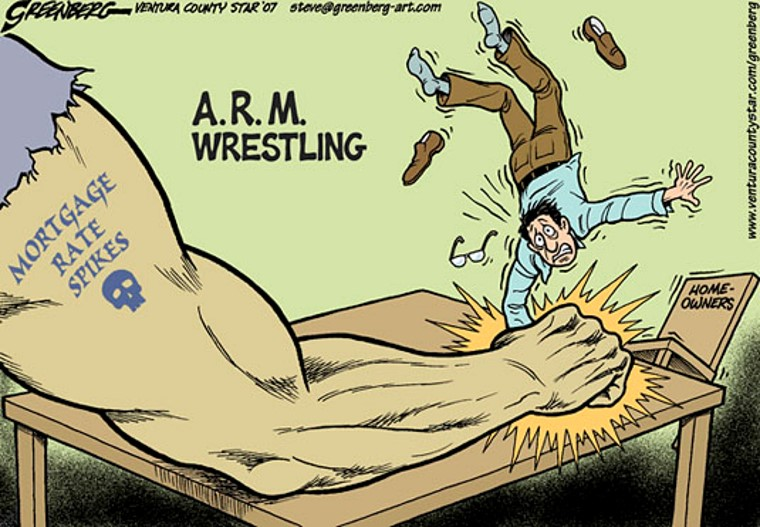
\includegraphics[width=\textwidth,height=.8\textheight,keepaspectratio]{Picture2.jpg}
\end{frame}

\begin{frame} 
	\frametitle{\LARGE{Background: Risk Overexposure}}
	\begin{itemize}
		\item Individual bankruptcies would not normally threaten the entire domestic economy, except...	
		\item ...Many banks and investment firms were heavily invested in derivatives and financial products based on these subprime mortgages. \pause
		\item \textbf{As borrowers default on their mortgages, this drags down the value of any products based on those mortgages. This implicates a wide array of complex financial products.} 
		
	\end{itemize}
\end{frame}

\begin{frame} 
	\frametitle{\LARGE{Background: Risk Overexposure}}
	\begin{itemize}
		\item This means the entire subprime mortgage market is a giant hot potato: these high risk investments are valued by the market in the present, but may not be in the future if their risks are realized in the form of default. \pause
		\item This means that brokers are encouraged to buy and sell these financial products quickly, to avoid being exposed to the risk for long. \pause
		\item \textbf{Most importantly, this means that any one firm dependent on these complex products going bankrupt will likely set off a chain reaction of bankruptcy.}
	\end{itemize}
\end{frame}



\begin{frame} 
	\frametitle{\LARGE{2008 Financial Crisis Begins}}
	At this point, the stage is set for the financial crisis as the subprime mortgage bubble is set to burst.
	\begin{itemize}
		\item Defaults start to occur, pulling down the stocks of investment firms that are heavily committed to products based on those loans.
		\item These defaults also hurt the banks issuing them, as they fail to recoup their investments. \pause
		\item Worried investors start to sell their assets in these banks and cash in on their \href{https://www.investopedia.com/terms/c/creditdefaultswap.asp}{credit default swaps}, reducing bank revenues at the same time.  	
	\end{itemize}
\end{frame}

\begin{frame} 
	\frametitle{\LARGE{2008 Financial Crisis Begins}}
	\begin{itemize}
		\item As these fears grow, investors sell their assets in these banks, leading to defaults of mortgage banks. \pause
		\item \textbf{Now it's not just individual borrowers who are defaulting, but banks themselves.}		
	\end{itemize}
\end{frame}

\begin{frame} 
	\frametitle{\LARGE{2008 Financial Crisis Spreads}}
	\begin{itemize}
		\item As banks start to default, the crisis spreads to other banks and investment firms that have substantial holdings of derivatives and complex financial products. \pause
		\item With the values of their assets plummeting, and firms cashing out of credit default swaps, these firms begin to implode.		
		\item These firms contain millions in assets from other banks, other Americans, and from other countries. 
		\item If they declare bankruptcy, or their stock value plummets, everyone gets collectively poorer...and this is exactly what happens.		
	\end{itemize}
\end{frame}

\begin{frame} 
	\frametitle{\LARGE{2008 Financial Crisis Spreads}}
	Why did this crisis spread throughout the economy, rather than staying contained to individual borrowers or specific banks?
	\begin{itemize}
		\item Recall what MBSs and financial derivatives did: spread the risk of subprime loans around to everyone who purchased any complex financial product based on those loans. \pause
		\item Now that the risk is realized, the threat of losses becomes systemic because of how widespread these financial products were.
		\item Investors see their net worth drop 50\% as the Dow Jones plummets. \pause
		\item In this market, practically everyone is exposed to the negative consequences of risky loans.
	\end{itemize}
\end{frame}

\begin{frame} 
	\frametitle{\LARGE{2008 Financial Crisis Keeps Spreading}}
	\begin{itemize}
		\item These investment firms and banks were themselves the targets of investment from both US and foreign corporations (including those in the EU) looking to improve their cash flow. \pause
		\item This means that these corporations, even those that are not banks themselves, are now exposed to the risks of the market.
		\item As the market contracts, the capital of these companies dries up, leaving them unable to pay their obligations and thus default.
		\item This leads to chains of bankruptcies and layoffs, \textit{even for firms which were not in the banking sector.}
	\end{itemize}
\end{frame}

\begin{frame} 
	\frametitle{\LARGE{2008 Financial Crisis: Falling Demand}}
	What is the Fed doing to try to stabilize the economy during this?
	\begin{itemize}
		\item The normal policy response would be for the Fed to cut interest rates, increasing the amount of money in the economy. \pause
		\item However, interest rates were already low (even after the 2004 increase), and so money was already saturating the system. \pause
		\item At the same time, money and value are disappearing with all the bankruptcies and defaults. 
	\end{itemize}
	At this point, the US economy is in free-fall.
\end{frame}

\begin{frame} 
	\frametitle{\LARGE{2008 Financial Crisis: General Responses}}
	Policy-makers recognize that swift action is needed.
	\begin{itemize}
		\item Both the US and EU implement emergency capital injections, along with the purchase of about a trillion dollars of troubled assets, propping up some banks. \pause
		\begin{itemize}
			\item The slogan ``too big to fail" originates here. \pause
		\end{itemize}
		\item The US also implements a stimulus package in 2009. \pause
		\item Meanwhile, the EU turns to austerity measures.
	\end{itemize}
\end{frame}

\begin{frame} 
	\frametitle{\LARGE{2008 Financial Crisis: US Response}}
	How did this play out in the American context? \pause
	\begin{itemize}
		\item The financial system in the US was effectively saved by the bailouts and government interventions (including TARP), though recovery takes years. \pause
		
		\item This crisis illustrated the problem of \textbf{moral hazard}, which had run rampant prior to the crisis, and was not entirely addressed in the aftermath. \pause
		
		\item \textbf{If a firm grows to the point where its failure would create systemic risk, it knows that governments will step in to prevent its failure, thereby encouraging risky behavior.} \pause
		
		\item Increased financial regulations may prevent specific risk-taking behaviors, but do not address this core problem.
		
		
	\end{itemize}
\end{frame}

\begin{frame} 
	\frametitle{\LARGE{2008 Financial Crisis: EU Impacts}}
	How did this play out in the European context? \pause
	\begin{itemize}
		\item As the financial crisis crosses the Atlantic, taking down firms and depressing the market, the EU's biggest problem becomes Greece. \pause
		\item Prior to the financial crisis, Greece sustained a large deficit paid off with shipping and tourism profits. \pause
		\item As global demand collapses due to the 2008 Financial Crisis, Greece can no longer pay off its deficit or finance its debt, and so it defaults.	\pause
		\item This launches the \textbf{Eurozone Crisis}, AKA the \textbf{European (Sovereign) Debt Crisis}.
	\end{itemize}
\end{frame}

\begin{frame} 
	\frametitle{\LARGE{EU Sovereign Debt Crisis}}
	This would not be a problem for the EU as a whole, except...
	\begin{itemize}
		\item Many other Eurozone states were financing Greek debt.
		\item This meant that a Greek default threatened the financial stability of the rest of the Eurozone. \pause
		\item Concurrently, the collapse of the real estate market due to subprime mortgages is driving up deficits in other European states. \pause
		\item The states most affected by the Great Recession are Greece, Portugal, Ireland, Spain, and Cyprus. 
	\end{itemize}
\end{frame}

\begin{frame} 
	\frametitle{\LARGE{EU Sovereign Debt Crisis}}
	
	\begin{itemize}
		\item These Eurozone states now desperately need credit, but cannot find it, as bailouts for that many states would be prohibitively difficult (and potentially not even fix structural issues anyway).\pause
		\item Those EU states that were least affected, especially Germany, argued for the need for structural reforms to EU economies to prevent the crisis from recurring.
	\end{itemize}
\end{frame}

\begin{frame} 
	\frametitle{\LARGE{EU Sovereign Debt Crisis Responses}}
	
	\begin{itemize}
		\item The EU, led by German Chancellor Angela Merkel, demanded that states like Greece adopt \textbf{austerity measures} in return for loans from entities like the European Central Bank. \pause
		\item These measures involved substantial tax increases and cuts to government spending. \pause
		\item Predictably, this led to substantial economic pain: in Greece and Spain unemployment was about 25\%, in Portugal and Iceland it was near 15\%. Economic demand collapses, making the recessions even worse.
	\end{itemize}
\end{frame}

\begin{frame}{\LARGE Austerity Reactions}
	\centering
	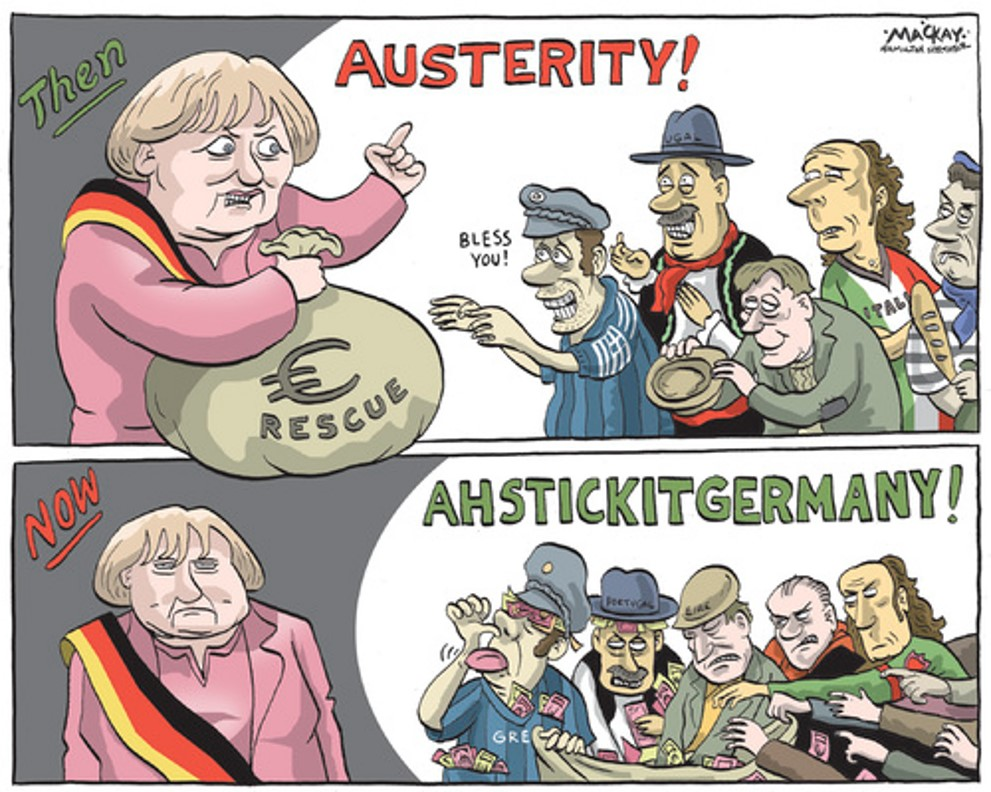
\includegraphics[width=\textwidth,height=\textheight,keepaspectratio]{Austeritycartoon.jpg}
\end{frame}

\begin{frame} 
	\frametitle{\LARGE{EU Sovereign Debt Crisis Resolution}}
	\begin{itemize}
		\item By the mid-2010s, EU bailout programs had officially ended and the crisis was officially over. \pause
		\item However, substantial doubts remained over whether austerity was the best policy option...
	\end{itemize}
\end{frame}

%https://databank.worldbank.org/source/2?series=NY.GDP.MKTP.KD.ZG&country=&l=en#advancedDownloadOptions
\begin{frame}{\LARGE US and EU Growth as \% of Annual GDP}
	\centering
	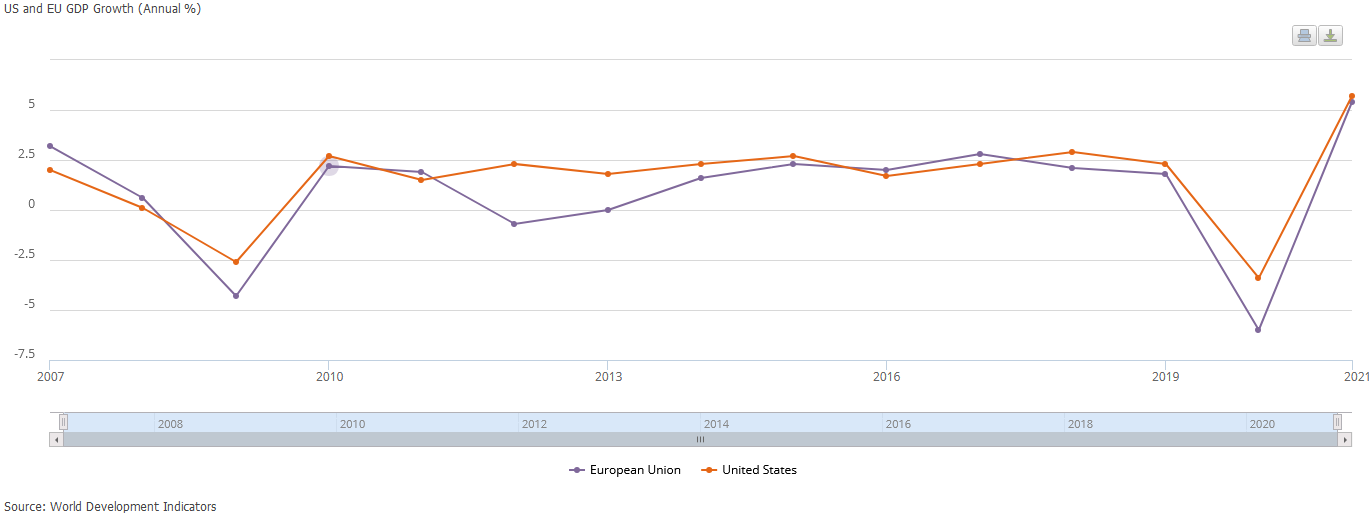
\includegraphics[width=\textwidth,height=\textheight,keepaspectratio]{WDIgdp.png}
\end{frame}

\begin{frame} 
	\frametitle{\LARGE{Legacies of Crisis}}
	\begin{itemize}
		\item Rise of backlash against globalization in both US and EU politics, influencing  electoral rhetoric and trends in the following years. 
		\item Brexit and its negative economic impacts.
		\item Rise of right-wing nationalist movements in the EU, often responding to economic concerns by advocating protectionism.	
	\end{itemize}
\end{frame}

\begin{frame} 
	\frametitle{\LARGE{Legacies of Crisis}}
	\begin{itemize}
		\item Rise of protectionist rhetoric from both parties in the US; withdrawal of US from trade agreements like the Trans-Pacific Partnership and Transatlantic Trade and Investment Partnership.
		\begin{itemize}
			\item TPP lived on in new form as the CPATPP, which did not include America. \pause.
		\end{itemize}
		\item Security concerns: is a more protectionist, less economically prosperous world going to encourage more adversarial relations between states?	
	\end{itemize}
\end{frame}



\begin{frame} 
	\frametitle{\LARGE{Review}}
	\begin{itemize}
		
			\item Relative currency values influence trade and investment. \pause  

			\item Governments manage currency through choosing among the monetary policy trilemma.  \pause

			\item Exchange rates are the relative values of currency to one another. \pause 

			\item Governments must commit to exchange rates, but may struggle to because of tradeoffs and domestic policy pressures. \pause 

			\item Currency manipulation is a heated debate, in US-China relations and elsewhere.
			
			\item Currency crises occur due to imbalances in the balance of payments.
			
			\item \href{https://www.youtube.com/watch?v=geoe-6NBy10}{Optional link reviewing the economic basis of these concepts}.
			

			
	
	\end{itemize}
\end{frame}



\end{document}
